\chapter{Method}\label{chp:method}

The method we will use to analyze and compare the different algorithms will be as follows.

We will create a large collection of randomly created instances/situations. Each of the algorithms will then be tasked with dividing the items. These allocations and division will then be compared directly in regards to the average score each agent gives their own bundle, and the total valuation for all agent combined. Because all algorithms will use the exact same items with the exact same valuations and agents, a comparison where one algorithms clearly outperforms the others wil be a clear sign that this algorithm is superior for that specific situation. The instances will be divided into a number of groups:

\begin{itemize}
    \item \textbf{Single Small Cake:} Instance with at least 1 indivisible item and 1 small cake (the indivisible items are dominant).
    \item \textbf{Single Large Cake:} Instance with at least 1 indivisible item and 1 large cake (the cake is dominant).
    \item \textbf{Multiple Cakes:} Instances with multiple divisible items. 
\end{itemize}

in addition to these metrics the algorithms will also be compared in regards to the time it takes to run the algorithm, and the general complexity/robustness the algorithm has. A very simple algorithm that perform just as well as, or close to, a complex algorithm can be considered a better algorithm. These evaluations are done in \autoref{chp:results} and finally presented in \autoref{chp:conclusion}. 


\clearpage
\section{Previous Solutions}\label{sec:previous-solutions}
\clearpage
\section{Our Solutions}\label{sec:our-solutions}



\subsection{Frozen Cake}\label{subsec:frozen-cake}
A simplification of the problem can be made by assuming the cake is \textit{frozen}, i.e. The cake is no longer divisible and must be allocated along with the indivisible items. This simplification naturally leads to an EF1 allocation with additive valuations. This does however remove the EFM guarantee as with a large cake, an agent with cake can now be envied, contradicting the rule of EFM. 

The algorithm for this is a direct copy of the algorithm desscribed in \cite{ef1}. Which is shown in \autoref{alg:frozen-cake}, pay attention to line \ref{alg:baseline:1}-\ref{alg:baseline:2}.

\begin{algorithm}
    \caption{Algorithm for Frozen Cake}\label{alg:frozen-cake}
    \begin{algorithmic}[1]
        \Require $n$ number of items, $m$ number of resources, $c_i$ cost of item $i$, $r_{ij}$ resource $j$ required by item $i$, $R_j$ resource $j$ available
        \Ensure $n \geq 0$ 
        \State $X \gets x$
        \State $N \gets n$
        \While{$N \neq 0$} \label{alg:baseline:1}
            \If{$N$ is even}
                \State $X \gets X \times X$
                \State $N \gets \frac{N}{2}$  \Comment{This is a comment}
            \ElsIf{$N$ is odd} \label{alg:baseline:2}
                \State $y \gets y \times X$
                \State $N \gets N - 1$
            \EndIf
        \EndWhile
    \end{algorithmic}
\end{algorithm}



\subsection{Frozen Cut Cake}\label{subsec:frozen-cut-cake}
A variation of the simplification in \autoref{subsec:frozen-cake} will be to assume the cake is cut into $n$ equally sized pieces. Again this simplification naturally leads to an EF1 allocation with additive valuations. 

We will further investigate how many pieces a cake should be cut in. A cake can potentially be cut into $\infty$ pieces, which will return the problem to the original problem. We are here instance focusing on a cake cut into a number of pieces $n$ that grows proprotinally with the number of agents. 

Again we use \autoref{alg:frozen-cake}, with the only difference being that the cake is cut into $n$ pieces. We will repeat the experiments with  $\frac{n}{2}$, $2n$ and $4n$ pieces of cut cake.








\begin{figure}
    \centering
    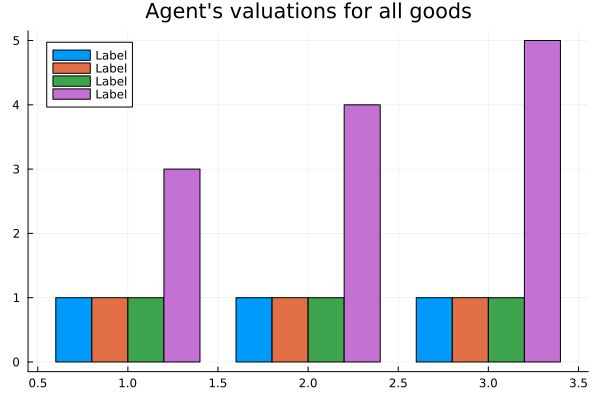
\includegraphics[width=0.8\textwidth]{assets/plots/visualize_instance.png}
    \caption{Visualization of agen's valuations in an instance, these valuations are used in the following figures.}
    \label{fig:visualize_instance}
\end{figure}

\begin{figure}
    \centering
    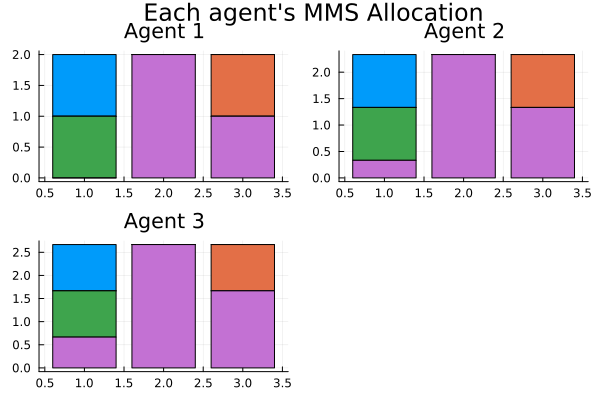
\includegraphics[width=0.8\textwidth]{assets/plots/visualize_mms_allocation.png}
    \caption{Visualization of each agents MMS Allocation for the mixed instance.}
    \label{fig:visualize_mms_allocation}
\end{figure}


\begin{figure}
    \centering
    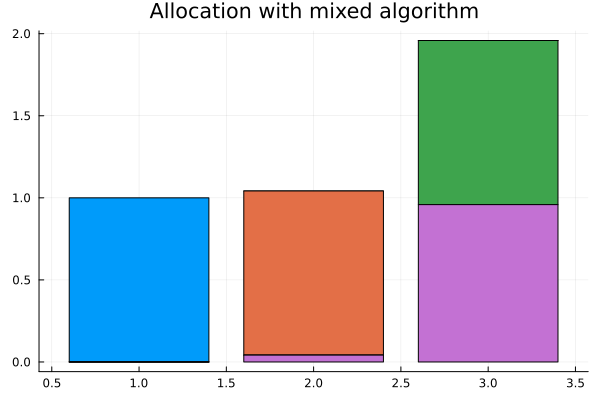
\includegraphics[width=0.8\textwidth]{assets/plots/visualize_mixed_allocation.png}
    \caption{Visualization of each agents MMS Allocation for the mixed instance.}
    \label{fig:visualize_mixed_allocation}
\end{figure}


\begin{figure}
    \centering
    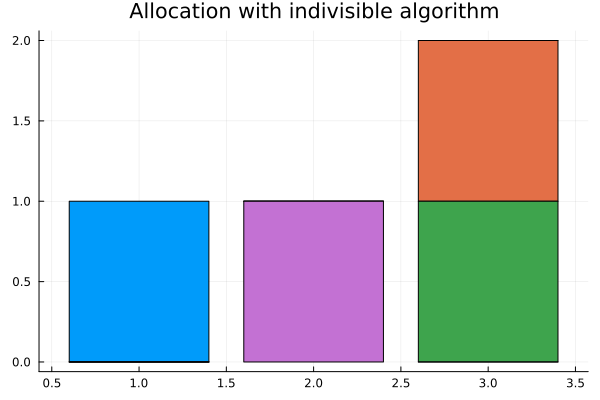
\includegraphics[width=0.8\textwidth]{assets/plots/visualize_indivisible_allocation.png}
    \caption{Visualization of each agents MMS Allocation for the mixed instance.}
    \label{fig:visualize_indivisible_allocation}
\end{figure}

\begin{figure}
    \centering
    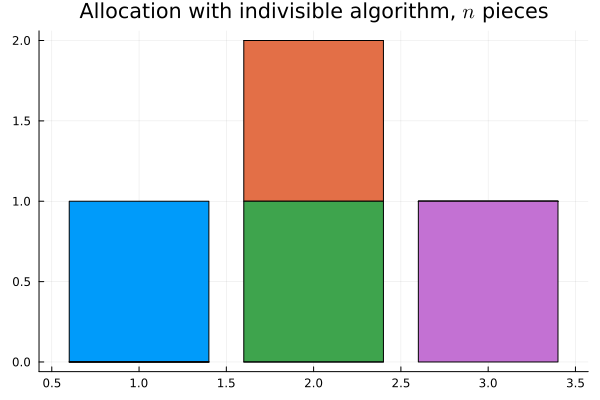
\includegraphics[width=0.8\textwidth]{assets/plots/visualize_indivisible_n_pieces_allocation.png}
    \caption{Visualization of each agents MMS Allocation for the mixed instance.}
    \label{fig:visualize_indivisible_n_pieces_allocation}
\end{figure}

